\chapter{Background \& \\Related Work}

\section{Fallacies in Argumetation}

The systematic study of logical fallacies can be traced back to Aristotle (350 BCE), who, in \textit{Sophistical Refutations} \cite{InternetClassicsArchive}, provided one of the earliest known classifications of flawed reasoning patterns. His foundational work laid the groundwork for subsequent inquiries into the nature and structure of fallacious reasoning. Several definitions of argument and fallacy have been introduced, in Figure \ref{fig:argument_fallacy}, we present the definitions of argument and fallacy as outlined by Copi et al. \cite{1CopiIrving}.

\begin{figure}[H]
    \centering
    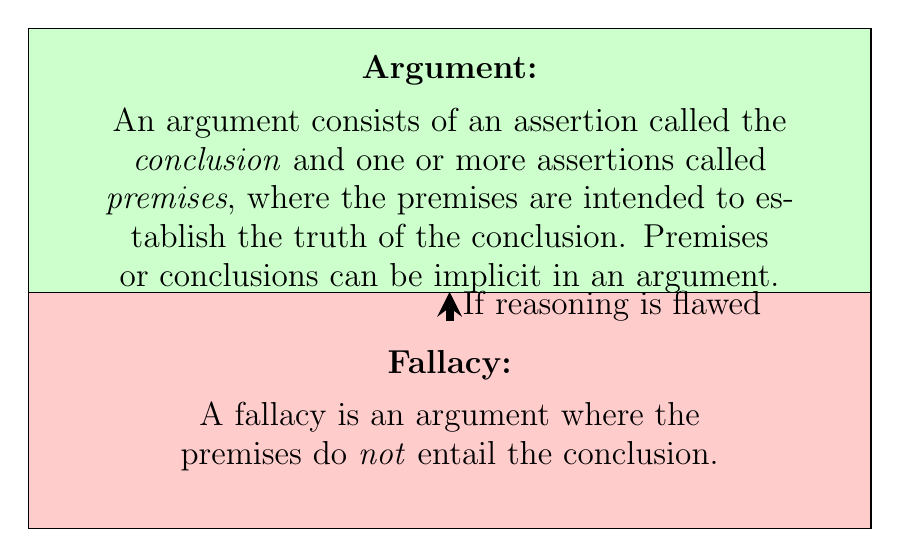
\begin{tikzpicture}[
        node distance=3cm, 
        every node/.style={align=center, font=\large},
        decision/.style={diamond, draw, fill=blue!20, text width=7cm, inner sep=5pt, minimum height=3cm},
        process/.style={rectangle, draw, fill=green!20, text width=10cm, inner sep=10pt, minimum height=3.5cm, anchor=north},
        fallacy/.style={rectangle, draw, fill=red!20, text width=10cm, inner sep=10pt, minimum height=3cm, anchor=south},
        arrow/.style={thick,->,>=stealth, line width=1mm}
    ]
    
    % Nodes
    \node (argument) [process] {\textbf{Argument:}\\[5pt] 
    An argument consists of an assertion called the \textit{conclusion} and one or more assertions called \textit{premises}, where the premises are intended to establish the truth of the conclusion. Premises or conclusions can be implicit in an argument.};
    
    \node (fallacy) [fallacy, below of=argument] {\textbf{Fallacy:}\\[5pt] 
    A fallacy is an argument where the premises do \textit{not} entail the conclusion.};
    
    % Arrows
    \draw [arrow] (argument.south) -- (fallacy.north) node[midway, right, font=\large] {If reasoning is flawed};
    
    \end{tikzpicture}
    
    \caption{Definitions of Argument and Fallacy by Copi et al. \cite{1CopiIrving}}
    \label{fig:argument_fallacy}
\end{figure}

% Throughout history, scholars have sought to refine, expand, and systematize Aristotle's work on logical fallacies. In the 19th century, \cite{whately1826} revisited Aristotle’s classification but maintained a relatively narrow scope, also listing only 13 fallacies. As the study of argumentation progressed, more comprehensive taxonomies emerged:

% \begin{itemize}
%     \item \cite{downes2003} expanded the classification to include 36 fallacies but omitted certain frequently occurring fallacies, such as the \textit{appeal to nature} and \textit{guilt by association}.
%     \item \cite{curtis2003} significantly increased the number of classified fallacies to 87 but did so without providing a structured hierarchical organization.
%     \item Later efforts by \cite{dowden2010}, \cite{bennett2012}, and \cite{hong2023} produced significantly broader taxonomies, with over 230 documented fallacies. These extensive lists, however, raise concerns about practical applicability, particularly in annotation and computational classification tasks.
% \end{itemize}

% While these taxonomies have considerably advanced our understanding of fallacious reasoning, they also introduce practical challenges. As noted by \cite{woods2004}, \cite{damer2008}, and \cite{hambiin2022}, the increasing volume of identified fallacies necessitates a structured classification system to facilitate detection and analysis. Without an effective organizational framework, the identification and practical application of fallacy classifications become arduous, particularly in domains such as legal argumentation, misinformation detection, and computational linguistics.

% \subsection{Definition of a Logical Fallacy}

% A logical fallacy is broadly defined as a form of reasoning that appears to be valid or persuasive but is, in reality, logically flawed \cite{woods2004, damer2008, hambiin2022}. While some fallacies stem from formal errors in logical structure, others arise from informal aspects such as relevance, ambiguity, or presumption.

% Some commonly recognized fallacies include:

% \begin{itemize}
%     \item \textbf{Circular Reasoning:} ``I am a great leader because I make great leadership decisions.'' This fallacy assumes the truth of the conclusion within the premises.
%     \item \textbf{False Analogy:} ``If we let students use calculators, they will never learn math, just as allowing pilots to use autopilot means they will never learn to fly.'' This fallacy draws an improper equivalence between two unrelated cases.
%     \item \textbf{Straw Man Argument:} ``People who support environmental regulations just want to ban all cars.'' This fallacy misrepresents an opposing argument to make it easier to attack.
% \end{itemize}

Logical fallacies are not confined to abstract philosophical discourse; they are can be found in various spheres of public communication, including:

\begin{itemize}
    \item \textbf{News media} Musi et al. \cite{musi2022fallacies}, where fallacious arguments are used to shape public perception.
    \item \textbf{Advertising} Danciu et al. \cite{danciu2014manipulative} , where misleading appeals are often employed to persuade consumers.
    \item \textbf{Propaganda and persuasion} Walton \cite{walton1997propaganda}, particularly in political and ideological discourse.
    \item \textbf{Political rhetoric} Blassnig et al. \cite{blassnig2019populism}, where fallacies are strategically utilized to influence public opinion.
    \item \textbf{Social media misinformation} Hidayat et al. \cite{hidayat2020logical}, where logical fallacies contribute to the rapid spread of false narratives.
\end{itemize}

Given the increasing role of digital platforms in shaping public discourse, the need to effectively identify and mitigate logical fallacies is greater than ever. Advancements in computational argumentation and artificial intelligence have opened new avenues for automating fallacy detection, making the study of fallacies not only a theoretical pursuit but also an essential component of contemporary information analysis.


\section{Fallacy Detection}

The field of logical fallacy detection has seen considerable progress in recent years, driven by the development of novel datasets, innovative methodologies, and advancements in Natural Language Processing (NLP). This section offers a chronological view of the main contributions to the field, highlighting significant milestones in dataset creation and the growing role of large language models (LLMs) in advancing research. By tracing these developments, we aim to provide a comprehensive understanding of how the field has evolved and where it stands today.
\par
In 2017, Habernal et al. \cite{habernalArgotarioComputationalArgumentation2017} were the first to identify the absence of datasets specifically focused on fallacious argumentation. To address this, they developed \textit{Argotario}, a gamified platform aimed at crowdsourcing annotated data for logical fallacies. The platform employed a competitive gameplay model, where participants either created or identified fallacious arguments created by other players. This approach resulted in a dataset encompassing five types of fallacies, including ad hominem and hasty generalization. Argotario functioned both as a data collection tool as well as an educational tool, raising public awareness about logical fallacies. The study demonstrated how gamification could effectively tackle the challenges of data annotation while simultaneously engaging users in meaningful ways.
\par


Building on these advancements, Da San Martino et al. (2019) \cite{dasanmartinoFineGrainedAnalysisPropaganda2019} introduced the \textit{PROPAGANDA} dataset. Unlike previous approaches that classified entire news articles as propagandistic, they focused on identifying propaganda techniques within text fragments of varying length. This shift allowed for a more interpretable analysis of how propaganda techniques are used in the written news context. The dataset included news articles annotated with 18 distinct propaganda techniques, with some of them being loaded language, name-calling, appeal to fear, and whataboutism, providing a comprehensive framework for studying these methods in detail.
The authors made several key contributions to the field. First, the dataset creation where they curated a corpus of news articles annotated at the fragment level by expert annotators. Second, they proposed two novel tasks: sentence-level classification, where a whole sentence is classified, and fragment-level classification, where a text span is identified as propagandistic alongside the corresponding propaganda technique. Finally, they developed a multi-granularity model that outperformed several strong BERT-based \cite{kenton2019bert} baselines, demonstrating its effectiveness in detecting propaganda at varying levels of granularity.
Their approach offered a more precise and explainable framework for analyzing propaganda in news articles.
\par

Vorakitphan et al. (2021) \cite{vorakitphanPROTECTPipelinePropaganda2022} introduced PROTECT (PROpaganda Text dEteCTion), propaganda detection and classification tool. PROTECT operates through a two-step pipeline. First, text snippets are identified as propagandistic, and second, these snippets are classified according to the specific propaganda technique employed. To achieve this, the system utilizes transformer-based language models, such as BERT and RoBERTa \cite{kenton2019bert, liu2019roberta}, and integrates semantic and argumentation features to improve classification accuracy. The system was evaluated using the PROPAGANDA dataset developed by Da San Martino et al. (2019) \cite{dasanmartinoFineGrainedAnalysisPropaganda2019}, demonstrating state-of-the art results. Beyond its technical capabilities, PROTECT was designed to be accessible to the public, featuring a user-friendly web interface that enables users to analyze submitted texts. This functionality serves an educational purpose, helping users recognize and understand the manipulative content in media. By providing a practical and accessible tool, this work made a significant contribution to the field, bridging the gap between technical research and public awareness. It highlights the potential of combining advanced NLP techniques with user-centric design to address complex challenges in media analysis and education.
\par

In 2021, Sahai et al. expanded the domain of fallacy detection to online discussions by constructing a dataset from Reddit.
The main contribution of this work was the construction of a large, balanced dataset of fallacies. The dataset is created using a two-stage annotation process. First, comments that explicitly mention fallacies were automatically collected from Reddit, and secondly they were manuallly validated via crowdsourcing. The final dataset consisted of eight common fallacies, including Appeal to Authority, Black-or-White Fallacy, Slippery Slope, and Hasty Generalization.
To classify these fallacies, the authors evaluated multiple models, including BERT-based fine-tuned classifiers and the multi-granularity networks introduced by Da San Martino et al. (2019) \cite{dasanmartinoFineGrainedAnalysisPropaganda2019}.
In addition, conversational context from the relevant Reddit threads was added which improved classification performance, highlighting the importance of discourse structure in fallacy detection.
This work built upon previous research in propaganda detection but unlike prior approaches that focused on detecting fallacies in journalistic articles, Sahai et al. (2021) focused on informal and unstructured online discussions, making their findings particularly relevant for misinformation analysis and online discourse quality assessment, while highlighting the importance of context in fallacy detection.
\par

Jin et al. (2022) \cite{jinLogicalFallacyDetection2022} introduced the LOGIC dataset, a large-scale benchmark for detecting 13 types of logical fallacies in natural language text with 2,449 samples. In addition, they propose LOGICCLIMATE, a specialized dataset for detecting fallacies in climate change claims. Their study highlights the difficulty of logical fallacy classification, as existing large language models (LLMs) exhibit limited performance, achieving only 53.31\% micro F1 at best.
The dataset includes fallacy types such as Faulty Generalization, Ad Hominem, Appeal to Emotion, False Causality, and Circular Claim, among others. The authors demonstrate that pretrained models (e.g., BERT, RoBERTa, DeBERTa, and Electra) struggle to generalize, especially to out-of-domain fallacies in climate discourse. To improve fallacy detection, they introduce a structure-aware classifier, which distills the argument structure by masking content words and focusing on logical patterns. This approach outperforms traditional LLMs by 5.46\% F1 on LOGIC and 4.51\% F1 on LOGICCLIMATE, highlighting the importance of formal logic structures in reasoning tasks.
Compared to previous work in propaganda detection (Da San Martino et al., 2019) and fallacy identification in Reddit discussions (Sahai et al., 2021), Jin et al. (2022) contribute a more comprehensive dataset covering multiple fallacy types, making it a significant benchmark for argument quality assessment. Their approach aligns with recent advances in reasoning-aware NLP, providing a foundation for future work in automated argument analysis andmisinformation detection.
\par
Alhindi et al. (2022) \cite{alhindiMultitaskInstructionbasedPrompting2022} proposed a unified multitask instruction-based prompting approach for fallacy detection that generalizes across multiple datasets. Unlike previous works, which focused on single-domain fallacy classification \cite{sahaiBreakingInvisibleWall2021} \cite{jinLogicalFallacyDetection2022}, their approach integrated five diverse datasets covering 28 fallacy types across different domains (news, dialogue, social media, fact-checking).
\begin{figure}[H]
\centering
\includegraphics[width=\textwidth]{graphics/Alhindi.png}
\caption{\textbf{Instruction-Based Prompting sceme} source: \cite{alhindiMultitaskInstructionbasedPrompting2022}}
\end{figure}
The authors fine-tuned a T5 transformer model \cite{raffel2020exploring} using instruction-based prompting, enabling it to recognize fallacies across various annotation schemes and linguistic structures. Their results demonstrate that multitask prompting significantly outperforms task-specific models, improving macro F1 scores by up to 16\% over single-dataset models and achieving better generalization to new domains. Moreover, they analyze the impact of model size, different prompting strategies, and dataset-specific challenges. Furthermore, they conducted a thorough error analysis, revealing the difficulty of the fallacy detection task by comparing an expert annotator's performance to the model's predictions and the dataset labels where the annotator agreed with the dataset's label in 75\% of the cases, with the model's predictions in 15\% of the cases whereas they provided a different label in 10\% of the cases.
Compared to earlier approaches that use BERT and RoBERTa-based classifiers for propaganda detection \cite{dasanmartinoFineGrainedAnalysisPropaganda2019} and logical fallacy identification \cite{jinLogicalFallacyDetection2022}, this work provides a more scalable and adaptable model. By leveraging multitask instruction tuning, their system captures cross-domain patterns in fallacious reasoning, making it a valuable contribution to automated argument assessment and misinformation analysis.
This study highlights the importance of unified instruction-based prompting for fallacy recognition in real-world settings, emphasizing the need for robust and generalizable models that can handle diverse fallacy types and linguistic structures.
\par
Goffredo et al. (2023) \cite{goffredoArgumentbasedDetectionClassification2023} focused on the automatic detection and classification of fallacies in political debates by extending an existing dataset and developing a transformer-based detection model.
Their first contribution was the expansion of the ElecDeb60To16 dataset, a corpus of U.S. presidential debates from 1960 to 2016, by adding the 2020 Trump-Biden debates and incorporating argumentative components (i.e., claims and premises) and the relations between these components (i.e., support
and attack). To detect and classify fallacies, the authors proposed MultiFusion BERT, a model architecture combining transformer-based text representations with argumentative features. Their model enhanced fallacy detection by integrating argumentative components and argumentative relations, which improved classification accuracy. Their experimental results showed that MultiFusion BERT outperforms standard transformer-based baselines such as BERT, RoBERTa, and DeBERTa.
This work emphasized in fallacy detection at the token level, making their approach more applicable to real-world scenarios where fallacious arguments are embedded in unstructured text.
By integrating argumentative structure into transformer-based architectures, this study outperformed previous methods. Nevertheless, their work cannot be easily generalized to real world scenarios since the argumentative features are not available in this context.
\par

Collectively, these studies demonstrate the evolution of fallacy detection, from gamified annotation platforms to sophisticated LLM-based methodologies.
Each contribution has addressed unique challenges, from scaling annotation processes to improving model interpretability and reasoning capabilities.
These advancements have not only deepened our understanding of logical fallacies but also expanded the applications of NLP in domains such as misinformation detection, argumentation analysis, and critical thinking education.

\section{Large Language Models (LLMs)}
Large Language Models (LLMs) have become a pillar of artificial intelligence in the modern era, using deep learning methods to generate and process human-like text. Based mainly on Transformer-based architectures \cite{vaswani2017attention}, these models have shown remarkable proficiency in natural language understanding, text generation, and reasoning tasks for a wide range of domains. As model sizes keep growing, pretraining objectives are refined, and fine-tuning methods are developed, LLMs are advancing the frontier of artificial intelligence in real-world applications.

This section gives a background to LLMs exploring the recent advancements ith focus in reasoning, and pointing out important models used for this research naemly, Falcon-Mamba-7B-Instruct, Meta-Llama-3.1-8B-Instruct, and Mistral-7B-Instruct-v0.3. 

LLM development has been in the forefront by the evolution of natural language processing (NLP) from statistical methods to deep learning approaches. Traditional methods worked well in basic NLP but had drawbacks of restricted context understanding. 
Then, though, came the Transformer architecture (Vaswani et al. \cite{vaswani2017attention}), which changed the game for NLP by using a self-attention mechanism to enable models to be trained on whole input sequences in parallel. This innovation made training much larger models possible and gave rise to the first generation of LLMs, including OpenAI's GPT \cite{radford2018improving} and Google's BERT \cite{kenton2019bert}.

LLMs have been developed through incremental advances in model scale, training data size, and computational efficiency.
Scaling laws research (Kaplan et al. \cite{kaplan2020scaling}) showed that model performance improves predictably with increased model size and training data. Subsequent models like GPT-3 (Brown et al., \cite{brown2020language}) and LLama (Touvron et al. \cite{touvron2023llama} 2023) used billion-parameter models, attaining excellent generalization on a wide range of NLP tasks.

One aspect of the Large Language Models that we are particualry interested in for this work, is their reasoning ability which has been a subject of extensive research. LLMs have been tested both for commonsense causality reasoning \cite{kıcıman2024causalreasoninglargelanguage}.
and abstract reasoning \cite{gendron2023large}. 
Yet, empirical research \cite{bubeck2023sparksartificialgeneralintelligence} has shown that LLMs, even the most recent versions like GPT-4, have inconsistencies in their reasoning.
\par

Commonsense reasoning evaluates the ability of an LLM to apply common sense while making decisions. The work of Kıcıman et al. (2023) \cite{kıcıman2024causalreasoninglargelanguage} and Talmor et al. (2020) \cite{talmor2022commonsenseqa20exposinglimits} has evaluated the performance of LLMs on causal understanding tasks. LLMs perform well on formal causal tasks but do poorly on real-world, complex scenarios involving implicit knowledge.
\par
Abstract reasoning, as studied by Gendron et al. (2023) \cite{gendron2023large} , which consists of finding and applying a general pattern from few data, argued that while models excel at syntactic pattern recognition, they often fail at true abstract generalization.
\par
Recently, Bubeck et al. \cite{bubeck2023sparksartificialgeneralintelligence}, despite their amazing performance in several tasks, has identified essential limitations in large language models (LLMs), specifically their consistency in reasoning tasks. Even the most advanced models (GPT-4) tend to derive contradictory conclusions from differences in prompts, suggesting that their reasoning is shaped more by the wording of inputs than by a deep understanding of logical principles.
\par
Building on these findings, we find it essential to examine the reasoning capabilities of LLMs in detecting logical fallacies, a task that requires a solid understanding of logical principles and the ability to detect flawed patterns of reasoning. Through an evaluation of LLMs' performance in fallacy detection tasks, we aim to understand their reasoning abilities and identify potential areas of improvement.
\par

\section{Chain of Thought}

Chain-of-Thought (CoT) prompting has greatly enhanced the reasoning ability of large language models (LLMs) by allowing them to decompose challenging problems into a series of intermediate steps. Conventional LLMs are usually poor at multi-step reasoning tasks, where they give straightforward but sometimes wrong responses because of the absence of systematic cognitive processes. CoT prompting overcomes this restriction by promoting the generation of explicit intermediate reasoning steps in models, thereby mimicking human-like logical reasoning.
\par
The concept of Chain-of-Thought (CoT) prompting was originally  defined originally by Wei et al. (2022) \cite{wei2022chain}, where they demonstrated that breaking complex issues into consecutive reasoning steps significantly improved the performance of large language models' (LLMs) on multi-step reasoning tasks. Their research demonstrated that if LLMs were prompted to provide intermediate reasoning steps, they were better on math word problems, logical reasoning tasks, and structured inference tasks of other natures. The innovation diverged from the classical "end-to-end" responding mode of LLMs, where generally immediate answers were produced by models without actually reasoning out the problem. The research demonstrated that CoT prompting particularly excelled on scaling laws, i.e., larger models gained greater benefits through reasoning chains compared to smaller models.
\par
Following this finding, follow-on research extended optimization of CoT prompting on varied reasoning tasks. Kojima et al. (2022) \cite{kojima2022large} in their effort to address the significant drawback in Wei et al.'s method which was the requirement for manually created exemplars, showed thta when LLMs were prompted to "think step by step," generated sizeable increases in logical consistency. The authors of this paper demonstrated that reasoning using CoT-type reasoning is effective on reasoning-trained models but can also automatically occur on very large LLMs.
\par
Zhou et al. (2023) \cite{zhou2023leasttomostpromptingenablescomplex} built upon the research of CoT prompting and formulated Least-to-Most (LtM) prompting. LtM tries to address CoT's problems in handling easier and harder tasks. Unlike standard CoT, which solves a problem step by step, LtM first breaks down a difficult task into easier, smaller components and solves them in turn, making use of prior responses along the way. This method substantially improves compositional generalization and multi-step reasoning performance compared to conventional CoT prompting on benchmarks like SCAN and GSM8K. Through hierarchical structuring of problem-solving, LtM improves the flexibility and development of reasoning in LLMs, bringing AI closer to human thinking abilities.
\par
The CoT prompting studies have shown that it is a highly effective technique for enhancing the reasoning capability of LLMs to enable them to resolve difficult multi-step problems more accurately and consistently. By breaking down problems into a series of intermediate steps, CoT prompting mimics human-like logical reasoning, providing a systematic problem-solving approach that can significantly improve the performance of LLMs on an extremely wide range of reasoning tasks. Therefore, we decided to use this technique in our work to explore how diffetent chain-of-thought techniques could enhance the capabilities of LLMs in detecting logical fallacies.